% =============================================================================
% sections/04_safety_systems.tex  -  Section 4: Safety Systems
% Teams: electronics + software / Status: scaffolded with stub content
%
% SCORING (0-10 pts):
%   1) Describe the safety system: architecture, time sequence, diagrams etc.
%   2) Prove the solution is robust: reliability analysis in a concise
%      engineering way.
%   3) Describe behaviour in an emergency - triggered by the system itself /
%      the operator / an external actor hitting the emergency button.
%      Ideally provide TEST RESULTS with figures/photos.
%
% Binding inputs:
%   - Jury feedback: the E-stop BUTTON CIRCUIT schematic was missing in the
%     Preliminary - it must appear in this section (see Emergency Stop).
%   - Page budget: ~3.5 pages.
%
% Ordering lives only here - leaf files under sections/design/safety/ have
% stable, unnumbered names and contain body content only.
% =============================================================================

\section{Safety Systems}
\label{sec:safety}

The rover implements a layered, defense-in-depth safety architecture
combining independent hardware and software mechanisms. Hardware-level
protection (Section~\ref{sec:estop}) is designed to remain functional
even in the event of a full software or main-computer failure, while
software-level mechanisms (Section~\ref{sec:sw-safety}) provide graceful
degradation before a hard shutdown becomes necessary.

\subsection{Emergency Stop}
\label{subsec:emergency_stop}
% =============================================================================
% sections/design/safety/emergency_stop.tex  -  Emergency Stop
% Teams: electronics + software (best guess - unconfirmed) / Status: stub
%
% Nested under "Safety Systems" (section-level subsection).
% =============================================================================

\begin{figure}[H]
    \centering
    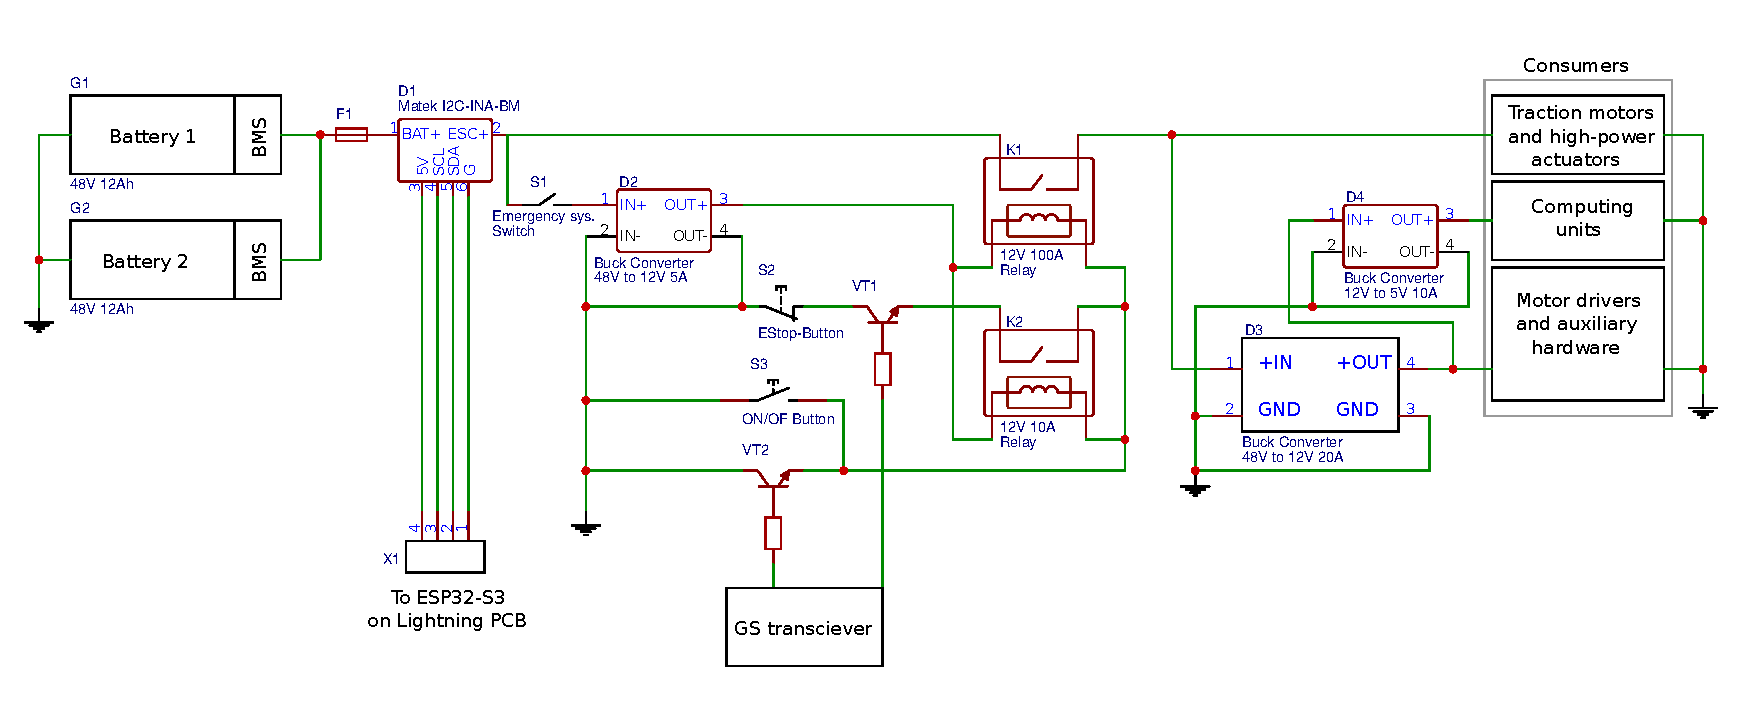
\includegraphics[width=\linewidth]{teams/electronics/figures/hardware_safety.pdf}
    \caption{Electrical schematic of the rover hardware safety system.}
    \label{fig:hardware_safety}
\end{figure}

The rover uses a dedicated hardware safety system independent of the main control electronics (Fig. \ref{fig:hardware_safety}). The primary power path is protected by a fuse (F1), while an INA-based module (D1) monitors battery voltage and current for state estimation and fault detection.

Power switching is implemented as a hardware self-latching circuit using relays K1 and K2, supplied by an independent 48 V-to-12 V converter (D2). The rover is powered on via the ON/OFF button (S3) or a remote command, while the relays maintain the powered state until an emergency stop is triggered.

Emergency shutdown can be triggered locally via the E-Stop button (S2) or remotely through an independent wireless channel. Both interrupt the relay latching circuit, immediately disconnecting rover power. As the emergency stop is implemented entirely in hardware, it operates independently of the onboard computer and software.

Rover status is indicated by a 360° industrial signal lamp mounted at its highest point. Four colors represent the operating state: orange (power on), green (manual mode), red (autonomous mode), and blue (wireless connection established).

The electronics enclosure is sealed with dedicated covers for removable modules, reducing dust and water ingress while ensuring reliable outdoor operation.



\subsection{Software Safety Systems}
\label{subsec:software_safety_systems}
% =============================================================================
% sections/design/safety/software_safety.tex  -  Software Safety Systems
% Teams: software (best guess - unconfirmed) / Status: stub
%
% Nested under "Safety Systems" (section-level subsection).
% =============================================================================

\todo[inline]{Description of how the rover is kept safe in software:
watchdogs and fault detection, safe-state transitions, behaviour on
communication/telemetry loss, collision-avoidance stop conditions, and any
automated responses to critical failures. Diagram of the software safety
architecture / state machine recommended. Include a reliability argument
for the solution.}

